\documentclass{standalone}
    %
    \usepackage{tikz,xcolor}
    \usetikzlibrary{shapes.geometric,arrows,positioning,fit}
    
\begin{document}
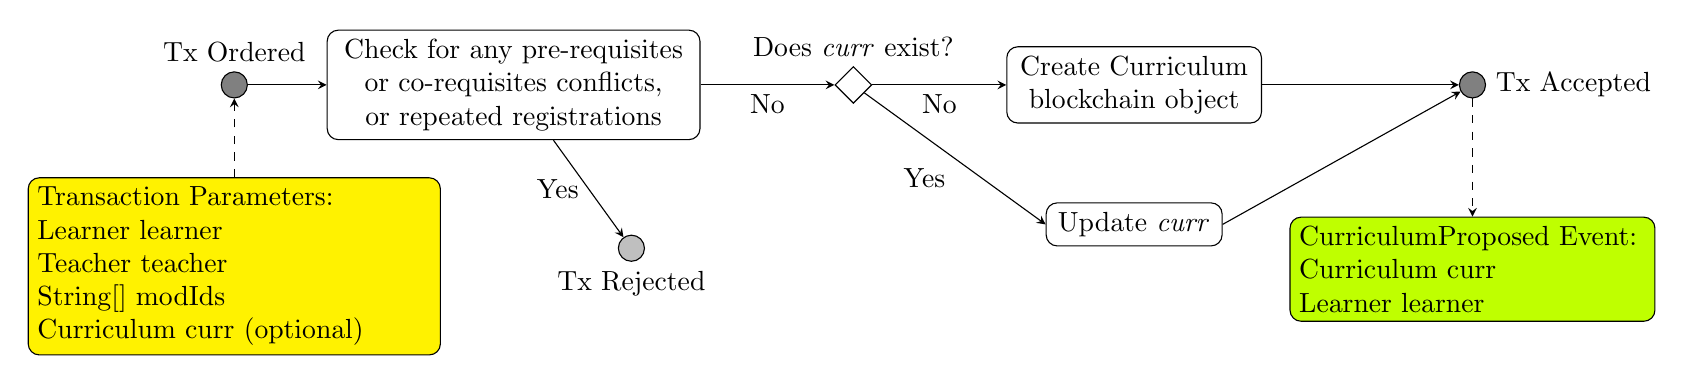
\begin{tikzpicture}[>=stealth,every node/.style={shape=rectangle,draw,rounded corners},]
	% create the nodes
	\node (start)[shape=circle, fill=gray, label=above:Tx Ordered] {};
    \node (param)[below =of start, text width=5cm, fill=yellow]{Transaction Parameters:\\Learner learner \\Teacher teacher\\ String[] modIds\\ Curriculum curr (optional)};
    \node (c1) [right =of start, text width=4.5cm, align=center]{Check for any pre-requisites or co-requisites conflicts, or repeated registrations};
    \node (c1b) [shape=diamond, sharp corners, right = 1.7cm of c1, label=above: Does \textit{curr} exist?]{};    
    \node (c1c) [right = 1.7cm of c1b, text width=3cm, align=center]{Create Curriculum blockchain object};    
	\node (c1d) [below =of c1c, text width=2cm, align=center]{Update \textit{curr}};        
    \node (stop1)[right = 2.5cm of c1c, shape=circle, fill=gray, label=right:Tx Accepted] {};
    \node (stop2)[below right = 1.25cm and -1cm of c1, shape=circle, fill=lightgray, label=below:Tx Rejected] {};        
    \node (event1)[below = 1.5cm of stop1, text width=4.4cm, fill=lime]{CurriculumProposed Event:\\ Curriculum curr \\ Learner learner };    

	% connect the nodes
	\draw[->, dashed] (param) to (start);
	\draw[->] (start) to (c1);
    \draw[->] (c1) -- node[draw=none, anchor=north] {No} (c1b);
    \draw[->] (c1) -- node[draw=none, anchor=east] {Yes} (stop2);
    \draw[->] (c1b) -- node[draw=none, anchor=north] {No} (c1c);  
    \draw[->] (c1b) -- node[draw=none, anchor=north east] {Yes} (c1d.west);      
    \draw[->] (c1c) to (stop1); 
	\draw[->] (c1d.east) to (stop1);        
	\draw[->, dashed] (stop1) to (event1);
    
\end{tikzpicture}
\end{document}
